% ## http://journals.plos.org/ploscompbiol/s/submit-now
% Template for PLoS
% Version 3.2 March 2016
%
% % % % % % % % % % % % % % % % % % % % % %
%
% -- IMPORTANT NOTE
%
% This template contains comments intended 
% to minimize problems and delays during our production 
% process. Please follow the template instructions
% whenever possible.
%
% % % % % % % % % % % % % % % % % % % % % % % 
%
% Once your paper is accepted for publication, 
% PLEASE REMOVE ALL TRACKED CHANGES in this file 
% and leave only the final text of your manuscript. 
% PLOS recommends the use of latexdiff to track changes during review, as this will help to maintain a clean tex file.
% Visit https://www.ctan.org/pkg/latexdiff?lang=en for info or contact us at latex@plos.org.
%
%
% There are no restrictions on package use within the LaTeX files except that 
% no packages listed in the template may be deleted.
%
% Please do not include colors or graphics in the text.
%
% The manuscript LaTeX source should be contained within a single file (do not use \input, \externaldocument, or similar commands).
%
% % % % % % % % % % % % % % % % % % % % % % %
%
% -- FIGURES AND TABLES
%
% Please include tables/figure captions directly after the paragraph where they are first cited in the text.
%
% DO NOT INCLUDE GRAPHICS IN YOUR MANUSCRIPT
% - Figures should be uploaded separately from your manuscript file. 
% - Figures generated using LaTeX should be extracted and removed from the PDF before submission. 
% - Figures containing multiple panels/subfigures must be combined into one image file before submission.
% For figure citations, please use "Fig" instead of "Figure".
% See http://journals.plos.org/plosone/s/figures for PLOS figure guidelines.
%
% Tables should be cell-based and may not contain:
% - tabs/spacing/line breaks within cells to alter layout or alignment
% - vertically-merged cells (no tabular environments within tabular environments, do not use \multirow)
% - colors, shading, or graphic objects
% See http://journals.plos.org/plosone/s/tables for table guidelines.
%
% For tables that exceed the width of the text column, use the adjustwidth environment as illustrated in the example table in text below.
%
% % % % % % % % % % % % % % % % % % % % % % % %
%
% -- EQUATIONS, MATH SYMBOLS, SUBSCRIPTS, AND SUPERSCRIPTS
%
% IMPORTANT
% Below are a few tips to help format your equations and other special characters according to our specifications. For more tips to help reduce the possibility of formatting errors during conversion, please see our LaTeX guidelines at http://journals.plos.org/plosone/s/latex
%
% For inline equations, please be sure to include all portions of an equation in the math environment.  For example, x$^2$ is incorrect; this should be formatted as $x^2$ (or $\mathrm{x}^2$ if the romanized font is desired).
%
% Do not include text that is not math in the math environment. For example, CO2 should be written as CO\textsubscript{2} instead of CO$_2$.
%
% Please add line breaks to long display equations when possible in order to fit size of the column. 
%
% For inline equations, please do not include punctuation (commas, etc) within the math environment unless this is part of the equation.
%
% When adding superscript or subscripts outside of brackets/braces, please group using {}.  For example, change "[U(D,E,\gamma)]^2" to "{[U(D,E,\gamma)]}^2". 
%
% Do not use \cal for caligraphic font.  Instead, use \mathcal{}
%
% % % % % % % % % % % % % % % % % % % % % % % % 
%
% Please contact latex@plos.org with any questions.
%
% % % % % % % % % % % % % % % % % % % % % % % %

\documentclass[10pt,letterpaper]{article}
\usepackage[top=0.85in,left=2.75in,footskip=0.75in]{geometry}

% Use adjustwidth environment to exceed column width (see example table in text)
\usepackage{changepage}

% Use Unicode characters when possible
\usepackage[utf8x]{inputenc}

% textcomp package and marvosym package for additional characters
\usepackage{textcomp,marvosym}

% fixltx2e package for \textsubscript
\usepackage{fixltx2e}

% amsmath and amssymb packages, useful for mathematical formulas and symbols
\usepackage{amsmath,amssymb}

% cite package, to clean up citations in the main text. Do not remove.
\usepackage{cite}

% Use nameref to cite supporting information files (see Supporting Information section for more info)
\usepackage{nameref,hyperref}

% line numbers
\usepackage[right]{lineno}

% ligatures disabled
\usepackage{microtype}
\DisableLigatures[f]{encoding = *, family = * }

% Remove comment for double spacing
\usepackage{setspace} 
\doublespacing

% Text layout
\raggedright
\setlength{\parindent}{0.5cm}
\textwidth 5.25in 
\textheight 8.75in

% Bold the 'Figure #' in the caption and separate it from the title/caption with a period
% Captions will be left justified
\usepackage[aboveskip=1pt,labelfont=bf,labelsep=period,justification=raggedright,singlelinecheck=off]{caption}
\renewcommand{\figurename}{Fig}

% Use the PLoS provided BiBTeX style
\bibliographystyle{plos2015}

% Remove brackets from numbering in List of References
\makeatletter
\renewcommand{\@biblabel}[1]{\quad#1.}
\makeatother

% Leave date blank
\date{}

% Header and Footer with logo
\usepackage{lastpage,fancyhdr,graphicx}
\usepackage{epstopdf}
\pagestyle{myheadings}
\pagestyle{fancy}
\fancyhf{}
\setlength{\headheight}{27.023pt}
\lhead{
\includegraphics[width=2.0in]{PLOS-submission.eps}}
\rfoot{\thepage/\pageref{LastPage}}
\renewcommand{\footrule}{\hrule height 2pt \vspace{2mm}}
\fancyheadoffset[L]{2.25in}
\fancyfootoffset[L]{2.25in}
\lfoot{\sf PLOS}

%% Include all macros below
\newcommand{\khalf}{\left(\frac{1}{2}\right)^{\delta_{ij}}}  % (1/2)^kronecker
\newcommand{\kkhalf}{\left(\frac{1}{2}\right)^{\delta_{ij} \delta_{kl}}}  % (1/2)^(kronecker * kronecker)
\newcommand{\Lspvl}{$\log_{10}$ SPVL}
\newcommand{\rzero}{{\mathcal R}_0}
\newcommand{\etal}{\textit{et al.}}
\newcommand{\tsub}[2]{#1_{{\textrm{\tiny #2}}}}
\newcommand{\PF}{\textrm{PF}}
\newcommand{\DS}{\textrm{DS}}
\newcommand{\WT}{\textrm{WT}}
\newcommand{\ET}{\textrm{ET}}
\newcommand{\DM}{\textrm{DM}}

\newcommand{\todo}[1]{\textbf{#1}}

%% END MACROS SECTION


\begin{document}
\vspace*{0.2in}

% Title must be 250 characters or less.
\begin{flushleft}
{\Large
\textbf\newline{Effects of Contact Structure on the Transient Evolution of HIV Virulence} % Please use "title case" (capitalize all terms in the title except conjunctions, prepositions, and articles).
}
%% short title: Epidemiological Structure and HIV Virulence Evolution
%% (53/70 characters)
\newline
% Insert author names, affiliations and corresponding author email (do not include titles, positions, or degrees).
\\
Sang Woo Park\textsuperscript{1}
Benjamin M. Bolker\textsuperscript{1,2,3,*}
\\
\bigskip
\textbf{1} Department of Mathematics \& Statistics,  McMaster University, Hamilton, Ontario, Canada
\\
\textbf{2} Department of Biology,  McMaster University, Hamilton, Ontario, Canada
\\
\textbf{3} Institute for Infectious Disease Research,  McMaster University, Hamilton, Ontario, Canada
\\
\bigskip

% Insert additional author notes using the symbols described below. Insert symbol callouts after author names as necessary.
% 
% Remove or comment out the author notes below if they aren't used.
%
% Primary Equal Contribution Note
%\Yinyang These authors contributed equally to this work.

% Additional Equal Contribution Note
% Also use this double-dagger symbol for special authorship notes, such as senior authorship.
%\ddag These authors also contributed equally to this work.

% Current address notes
%\textcurrency Current Address: Dept/Program/Center, Institution Name, City, State, Country % change symbol to "\textcurrency a" if more than one current address note
% \textcurrency b Insert second current address 
% \textcurrency c Insert third current address

% Deceased author note
%\dag Deceased

% Group/Consortium Author Note
%\textpilcrow Membership list can be found in the Acknowledgments section.

% Use the asterisk to denote corresponding authorship and provide email address in note below.
* bolker@mcmaster.ca

\end{flushleft}
% Please keep the abstract below 300 words
% current is 296
\section*{Abstract}
Early in an epidemic, high densities of susceptible hosts
select for relatively high parasite virulence; later in the epidemic,
lower susceptible densities select for lower virulence.
Thus over the course of a typical epidemic the average virulence 
of parasite strains increases initially,
peaks partway through the epidemic, then declines again.
However, precise quantitative outcomes, such as the peak virulence reached
and its timing, may depend sensitively on epidemiological details. 
Fraser \emph{et al.}
proposed a model for the eco-evolutionary
dynamics of HIV that incorporates
the tradeoffs between transmission and virulence (mediated by
set-point viral load, SPVL) and their heritability between
hosts. Their models use implicit equations to
capture the effects of partnership dynamics that are at the core of 
epidemics of sexually transmitted diseases. 
Our models combine HIV virulence tradeoffs with a range of
contact models, modeling partnership formation and
dissolution and allowing for individuals to transmit disease outside
of partnerships. We assess summary statistics such as the peak virulence
(corresponding to the minimum expected time of progression to AIDS) across
models for a range of 
parameters applicable to the HIV epidemic in sub-Saharan Africa.
Although virulence trajectories are broadly similar
across models, the timing and magnitude of the 
virulence peak vary
considerably.
Previously developed implicit models predicted 
lower virulence and slower progression
at the peak (a minimum of 15 years to
progress to AIDS) compared both to more realistic models
and to simple random-mixing models with no partnership structure
at all (both with a minimum of $\approx$ 7.25 years to progress to AIDS).
In this range of models, the simplest random-mixing structure best
approximates the most realistic model; this
surprising outcome occurs because the dominance of extra-pair
contact in the realistic model swamps the effects of
partnership structure.

% Please keep the Author Summary between 150 and 200 words
% Use first person. PLOS ONE authors please skip this step. 
% Author Summary not valid for PLOS ONE submissions.   
\section*{Author Summary}

%% 199 words

Pathogens such as HIV can evolve rapidly when the environment changes.
Such changes include decreases in the probability that an infectious
contact (such as a sneeze for a respiratory disease, or an unprotected
sex act for a sexually transmitted disease) encounters an uninfected,
susceptible person and thus has a chance to transmit the
pathogen. Disease spread during an epidemic reduces the fraction of
susceptible people in the population and thus changes the direction of
parasite evolution.  While researchers have explored these
evolutionary dynamics with simulations, their models have neglected
important processes such as people entering and leaving sexual
partnerships. We compared several evolutionary models that include
partnership dynamics and sexual contact outside of stable
partnerships. Models of intermediate complexity predicted lower
virulence over the course of the epidemic (a minimum of 15 years to
progress to AIDS) than either more realistic models or simple models
without any partnership structure at all (both approx. 7.25 years to
progress to AIDS), because sexual contact outside of stable
partnerships tended to wash out the effects of contact
structure. The large effect of epidemiological details on evolutionary
dynamics suggests that researchers trying to predict the evolution of
pathogens should proceed with caution.

\linenumbers

% Use "Eq" instead of "Equation" for equation citations.
\section*{Introduction}

The evolution of pathogen virulence has both 
theoretical and, potentially, practical
importance. In general, evolutionary theory suggests that
pathogens with higher reproduction numbers ($\rzero$) --- that is, the number of secondary infections caused by a single infected host over the course of its infectious period --- will tend to increase in prevalence relative to strains with lower reproductive ratios.
Pathogens can increase their reproduction numbers either
by increasing their transmission rate, 
the rate (per infected host) at which they
infect new hosts, or by decreasing their clearance or disease-induced
mortality rate, the rate
at which hosts recover or die from disease.
The \emph{trade-off theory} \cite{alizon_virulence_2009} postulates that
transmission and disease-induced mortality rates are both driven by the rate at which
the pathogen exploits host resources for within-host reproduction, 
and that pathogen
evolution will thus strike a balance between the
pathogen's rate of transmission
to new hosts and its rate of killing its host (or of provoking
the host's immune system to eliminate it).
Some biologists have criticized the tradeoff theory
\cite{EbertBull2003,alizon_adaptive_2015}, but others have
successfully applied it to a variety of host-pathogen systems \cite{Dwyer+1990,mackinnon1999genetic,jensen2006empirical,deroode2008virulence}.

Fraser \etal\ have applied these ideas to HIV,
showing that the virus appears to satisfy the prerequisites of
the tradeoff theory.
The \emph{set-point viral load} (SPVL: i.e., the
characteristic virus load measured in blood during the intermediate
stage of infection) is a measurable proxy for the rate of HIV within-host
reproduction. Higher viral loads are correlated with 
shorter progression times (higher virulence).
Studies of discordant couples --- stable
sexual partnerships with one infected and one uninfected partner --- %
have shown that SPVL is (1) correlated with faster transmission
(the time to infection of the uninfected partner is shorter when
their partner has a higher SPVL) and (2) heritable
(when the uninfected member of
the couple does become infected, their SPVL is similar to their
partner's).
Furthermore, the rate of transmission increases with
increasing SPVL (and hence with decreasing progression time)
but with a decreasing slope as progression time decreases,
fulfilling the requirements of the tradeoff theory
 \cite{Fraser+2007}.
Subsequent studies
\cite{shirreff_transmission_2011,herbeck_hiv_2014,herbeck_evolution_2016} used these data to
parameterize mechanistic models of HIV virulence evolution, suggesting
that HIV invading a novel population would initially evolve increased
virulence, peaking after approximately 100-200 years and then declining
slightly to a long-stable virulence level.

The work of Shirreff \etal\ \cite{shirreff_transmission_2011}, and particularly the predicted transient peak in HIV virulence midway through the epidemic,
highlights the importance of interactions between epidemiological and
evolutionary factors \cite{day_virulence_2004,alizon_price_2009}.
However, despite these studies' attention to detail at the individual
or physiological level, the contact structures used in these
models are relatively simple.

As we discuss in detail below,
existing models of HIV eco-evolutionary dynamics either use implicit
models that incorporate the average effects of within-couple sexual
contact --- without representing the explicit dynamics of pair
formation and dissolution or accounting for extra-partnership contact %
--- or use an agent-based formulation with parameters that effectively
lead to random mixing among infected and uninfected individuals. Here
we explore the effects of incorporating \emph{explicit}
contact structure in eco-evolutionary models.

Because our main goal is to explore how conclusions about virulence
evolution depend on the way in which contact structure
is modeled, we consider a series of
models with increasing levels of complexity in the contact
structure, but simplify some of the other epidemiological
processes (such as the within-host life history of HIV). 
We evaluate our models
across a wide range of parameters, using a Latin hypercube design; for
each model run, we compute a set of metrics 
that summarize the evolutionary trajectory of SPVL
over the course of the epidemic.

\section*{Materials and Methods}

\subsection*{Infection dynamics}

As in Shirreff \etal\ \cite{shirreff_transmission_2011}, our models
explicitly track the evolution of mean $\log_{10}$ SPVL
(which we denote as $\alpha$), rather than the rate of progression to
AIDS itself (hereafter ``virulence'' will refer either to the SPVL, or
to the rate of progression to AIDS; these two quantities are
deterministically linked in the model).  
In contrast to Shirreff \etal, we use a
single-stage disease model instead of accounting explicitly for
progression through the three main stages of HIV infection (primary,
asymptomatic, and disease), and we use an exponentially
distributed infectious period instead of a more realistic
Weibull-distributed infectious period; we show below that our results
are not overly sensitive to this simplification. We account for
varying transmission rates and durations of each disease stage by
summing the durations of three stages (again based on Shirreff \etal's
model) and taking the duration-weighted average of transmission rates
of three stages. Thus the within-couple transmission rate, $\beta$,
for our models is given by:
\begin{equation}
\beta (\alpha) = \frac{D_P \beta_P + D_A (\alpha) \beta_A (\alpha) + D_D \beta_D}{D_P + D_A (\alpha) + D_D},
\end{equation}
where the duration of infection ($D_P$ and $D_D$) and rate of transmission ($\beta_P$ and $\beta_D$) of the Primary and Disease stages
of infection are independent of the host's SPVL
(Table~\ref{table:parmsTable} gives definitions, units, and values for all parameters).
. Following Shirreff \etal, the duration of infection ($D_A$) and rate of transmission ($\beta_A$) for the Asymptomatic stage are Hill functions of the SPVL:

\begin{equation}
\begin{split}
D_A(\alpha) &= \frac{\tsub{D}{max} D_{50} ^{D_k}}{V_\alpha ^{D_k} + D_{50}^{D_k}}, \\
\beta_A(\alpha) &= \frac{\tsub{\beta}{max} V_\alpha ^ {\beta_k}}%
{V_\alpha^{\beta_k} + \beta_{50} ^{\beta_k}},
\end{split}
\label{eq:hillfuns}
\end{equation}
where $V_{\alpha} = 10^\alpha$. 

The uncoupled and extra-couple transmission rates (i.e., the rates of
transmission among people outside of a stable partnership, or between
people inside of a stable partnership and people other than their
partner) are scaled by
multiplying the within-couple transmission rate $\beta$ by the contact
ratios $c_u/c_w$ and $c_e/c_w$ (see Appendix S1). Simplifying the model
of HIV pathogenesis from three stages to a single stage could affect
our conclusions about the evolution of virulence (e.g. Kretzschmar and
Dietz \cite{kretzschmar_effect_1998} show that pair formation dynamics
and multiple stages of infectivity have interactive effects on
$\rzero$). However, our simplified model produces results that are
qualitatively similar to those of Shirreff \etal's
\cite{shirreff_transmission_2011} model; when our model is calibrated
to have a similar initial epidemic growth rate $r$, the peak
\Lspvl\ occurs at the same time ($\approx 200$ years) but slightly
higher (4.6 \Lspvl\ vs. 4.3 \Lspvl: \figurename~\ref{fig:panel3}).

\begin{figure}[!ht]
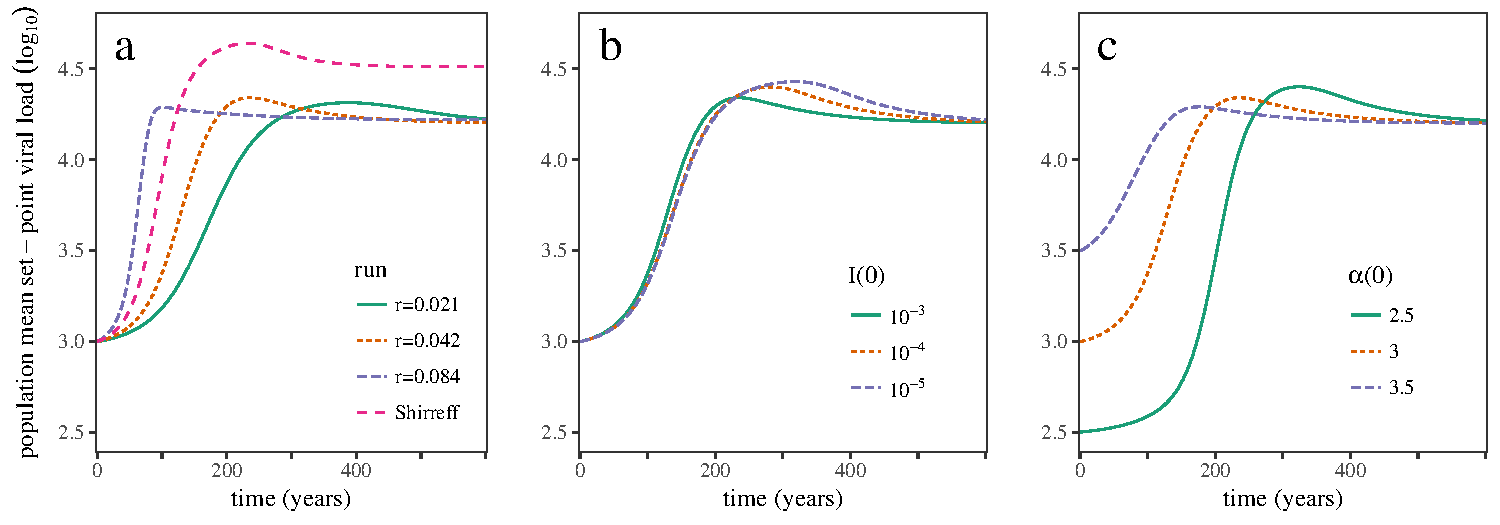
\includegraphics[width=\textwidth]{../figures/fig1.pdf}
\caption{{\bf Baseline dynamics.}
Time series of mean population \Lspvl\ using mean parameters. Each initial condition was varied independently while rest were kept constant in order to test their effects on the transient dynamics of virulence evolution. Note that the initial condition has negligible effect on equilibrium virulence.
(a) Contrast between the three-stage Shirreff model and the single-stage model calibrated to varying initial exponential growth rates, $r$. achieved quicker.
(b) Effects of varying initial infectious density $I(0)$.
(c) Effects of varying initial mean virulence $\alpha(0)$.
The $r=0.042$ (orange, dotted) curve in panel (a), calibrated to match the epidemic dynamics of Shirreff \etal's model \cite{shirreff_transmission_2011}, shows that our simplified model can produce similar virulence trajectories. 
Although the virulence dynamics are sensitive to each initial condition, we are still able to achieve similar qualitative dynamics dynamics across a range of parameters. 
For fair comparison, we hold them constant in our simulations.}
\label{fig:panel3}
\end{figure}

\subsection*{Mutation}

Like Shirreff \etal\ \cite{shirreff_transmission_2011} we incorporate a between-host mutation process in the SPVL. We simplify Shirreff \etal's evolutionary model by using a one-to-one genotype-phenotype mapping rather
than allowing for variation in phenotypes of a single genotype.
The mutational process in our model is directly taken from Shirreff \etal. Over the course of infection, mutation occurs within the host. However, it is assumed that SPVL of the strain transmitted by an infected individual is determined by the SPVL at the time of infection and is not further affected by within-host mutation. Instead, the mutational effect takes place in a single
step at the time of transmission. First, the distribution of \Lspvl\ is discretized into a vector:
\begin{equation}
\alpha_i = \tsub{\alpha}{min} + (\tsub{\alpha}{max} - \tsub{\alpha}{min})\frac{i-1}{n-1} \qquad i = 1,2,3, \dots n.
\end{equation}
We have experimented with varying degrees of discretization in the strain distribution (i.e., values of $n$); in our model runs comparing results with Shirreff \etal\ \cite{shirreff_transmission_2011} (\figurename~\ref{fig:panel3}) we use $n=51$ (i.e. a bin width of 0.1 \Lspvl\ for $\alpha$), but reducing $n$ to 21 (bin width = 0.25 \Lspvl) makes little difference; we use this coarser grid for all other simulations reported.

We construct an $n$ by $n$ mutational matrix, $M$ --- which is multiplied with the transmission term ---  so that $M_{ij}$ is the probability that a newly infected individual will have \Lspvl\ of $\alpha_j$ given that the infector has \Lspvl\ of $\alpha_i$. Finally, the probabilities are normalized so that each row sums to 1:
\begin{equation}
M_{ij} = \frac{\Phi(\alpha_j + d/2;i) - \Phi(\alpha_j - d/2;i)}{\Phi(\tsub{\alpha}{max} + d/2;i) - \Phi(\tsub{\alpha}{min} - d/2;i)},
\end{equation}
where $\Phi(x;i)$ is the Gaussian cumulative distribution function with mean $\alpha_i$ and variance of $\sigma_M^2$, and $d = (\tsub{\alpha}{max} - \tsub{\alpha}{min})/(n-1)$. Transmission rate and disease induced mortality rates are discretized as well:
\begin{equation}
\begin{aligned}
\beta_i &= \beta(\alpha_i),\\
\lambda_i &= \frac{1}{D_P + D_A (\alpha_i) + D_D}.
\end{aligned}
\end{equation}

\subsection*{Contact structure and partnership dynamics}

We developed seven multi-strain evolutionary models covering a gamut including Champredon \etal's relatively realistic \cite{champredon_hiv_2013} and Shirreff \etal's relatively simple \cite{shirreff_transmission_2011} contact structures, each of which is based on different assumptions regarding contact structure and partnership dynamics. Specifically, we focus on the effects of the assumptions of (1) instantaneous vs. non-instantaneous partnership formation; (2) zero vs. positive extra-partnership sexual contact and transmission; and (3) homogeneous vs. heterogeneous levels of sexual activity on the evolution of mean \Lspvl.

Our first four models consider explicit partnership dynamics and are based on Champredon \etal's model \cite{champredon_hiv_2013}. The first two (``pair-formation'' or ``pairform'' for short) assume non-instantaneous partnership formation (i.e. individuals spend some time uncoupled, outside of partnerships) and consist of five states that are classified by infection status and partnership status. $S$ is the number of single (uncoupled) susceptible individuals, and $I$ is the number of single infected individuals. $SS$ is the number of concordant negative (susceptible-susceptible) couples, $SI$ is the number of serodiscordant (susceptible-infected) couples, and $II$ is the number of concordant positive (infected-infected) couples. The first (``pairform+epc'') includes extra-partnership contact (with both uncoupled individuals and individuals in other partnerships) whereas the second (``pairform'') only considers within-couple transmission. 

The next two models, which are intended to bridge the gap between models with fully explicit pair-formation dynamics and the simpler, implicit models used by Shirreff \emph{et al.} \cite{shirreff_transmission_2011}, assume instantaneous partnership formation (``instswitch''). The compartmental structure thus omits the single states $S$ and $I$, comprising only the three partnered states: $SS$, $SI$, and $II$. Like the first two models, this pair of models differs in their inclusion of extra-pair contact: the third model (``instswitch+epc'') includes extra-partnership contact (now only with individuals in other partnerships, since uncoupled individuals do not exist in this model) while the fourth (``instswitch'') only considers within-couple transmission. Although these models can also be implemented
by setting the partnership formation rate of the explicit partnership models to a high value (and we have tested that both methods in fact produce same results), we model instantaneous partnership formation models independently in order to avoid scaling of partnership formation rate during model calibration affecting the virulence trajectory.

The fifth and sixth models represent extreme simplifications of sexual partnership dynamics.  One (``implicit'') is an implicit serial monogamy model based on the epidemiological model used by Shirreff \etal\ \cite{shirreff_transmission_2011}. It is actually a random mixing model that explicitly tracks only the total number of susceptible and infected individuals. However, to reflect the effect of partnership structure, it uses an adjusted transmission rate derived from an approximation of the basic reproduction number of a serial monogamy model with instantaneous pair formation \cite{hollingsworth_hiv1_2008}. The second model of this pair (``random'') is a simple random-mixing model.

Lastly, we add a model of heterogeneity in sexual activity to the pairform+epc model (``hetero''). Individuals are divided into different risk groups based on the sexual activity level; we scale all aspects of sexual activity, assuming that sexual activity level in both within- and extra-couple contacts is directly proportional to number of non-cohabiting (extra-couple and uncoupled) partners per year \cite{omori2015dynamics} (see Appendix S1). We assume random activity-weighted mixing between risk groups \cite{may_transmission_1988}. While this model lacks some 
important elements, such as age-structured mixing patterns, needed for realistic models of HIV transmission in sub-Saharan Africa, it represents a first step toward assessing the effects of epidemiological complexity. As even the models shown here push the limits of compartmental-based models (the heterogeneity model comprises 24530 coupled ordinary differential equations), adding further complexity will probably require a shift to an agent-based model framework, as well as considerable effort in model calibration \cite{herbeck_hiv_2014,delva_connecting_2016}.

The pairform+epc and heterogeneous models use the basic epidemiological framework of Champredon \etal \cite{champredon_hiv_2013}. Individuals in single compartment acquire a partner at a rate $\rho$, and partnerships dissolve at a rate $c$. Infected individuals in a discordant partnership infect their susceptible partner at a rate $\beta$ (within-couple transmission rate) and susceptible individuals outside the partnership at a rate $c_e$ (extra-couple transmission rate). Likewise, a single infected individual can infect any susceptible individuals at a rate $c_u$ through uncoupled mixing. Extra-couple and uncoupled transmission are modeled in the same way as in Champredon \etal's model. All the details have been adapted to a multi-strain scenario, so that we track (for example) a matrix 
$II_{ij}$ that records the number of concordant, HIV-positive couples in which the two partners have \Lspvl\ of $\alpha_i$ and $\alpha_j$. 
The second through fourth models (pairform, instswitch+epc, instswitch) are derived from the base model by simplifying epidemiological processes (partnership formation and uncoupled/extra-couple contact: see Appendix S1).

\subsection*{Latin hypercube sampling}

Despite considerable effort \cite{hollingsworth_hiv1_2008,champredon_hiv_2013}, the parameters determining the rate and structure of sexual partnership change and contact are still very uncertain; this led Champredon \etal\ \cite{champredon_hiv_2013} to adopt a Latin hypercube sampling (LHS) strategy \cite{blower_drugs_1991} that evaluates model outcomes over a range of parameter values. In order to make sure that our comparisons among models apply across the entire space of reasonable parameter values, and in order to evaluate the differential sensitivity of different model structures to parameter values, we follow a similar protocol and perform LHS over a parameter set including both the early- and late-stage transmission and duration parameters ($\beta_P$, $D_P$, $\beta_D$, $D_D$) and contact/partnership parameters ($\rho$, $c$, $c_u/c_w$, and $c_e/c_w$). For the heterogeneity model, the mean and squared coefficient of variation (CV) for the number of non-cohabiting partners are sampled as well. We do not allow for uncertainties in parameters that are directly related to the evolutionary process ($\tsub{\beta}{max}$, $\beta_{50}$, $\beta_k$, $\tsub{D}{max}$, $D_{50}$, $D_k$, $\sigma_M$), instead using Shirreff \etal's point estimates throughout \cite{shirreff_transmission_2011}.

Latin hypercube sampling is done as in Champredon \etal\ \cite{champredon_hiv_2013}. For each parameter, $z$, its range is divided into $N = 1000$ equal intervals on a log scale:
\begin{equation}
z_i = \exp\left(\log(\tsub{z}{min}) + [\log(\tsub{z}{max}) - \log(\tsub{z}{min})] \frac{i-1}{N-1}\right) \qquad i = 1, 2, 3, \dots,N.
\end{equation}
Random permutations of these vectors form columns in a sample parameter matrix; each row contains a different parameter set that is used for one simulation run.

Table~\ref{table:parmsTable} gives the ranges of the model parameters used for LHS. Parameter ranges regarding contact and partnership dynamics ($\rho$, $c$, and $c_e/c_w$) are taken from Champredon \etal\ \cite{champredon_hiv_2013}, whereas those regarding infection ($\beta_P$, $D_P$, $\beta_D$, and $D_D$) are taken from Hollingsworth \etal\ \cite{hollingsworth_hiv1_2008}. The remaining parameters are taken from Shirreff \etal\ \cite{shirreff_transmission_2011}.

%Tables need to be placed after the first paragraph in which they are cited.

\begin{table}[h!]
\caption{Parameter ranges/values.  Values of $c$ and $\rho$ are doubled from those given by Champredon \etal\ because we keep track of individuals in the model, while they keep track of couples. Starred (*) parameters (used in \figurename~\ref{fig:panel3}), and descriptions of Hill function coefficients, are taken from \cite{shirreff_transmission_2011}.}
\centering
\begin{tabular}{c p{2in} c l}
\hline 
Notation & Description & Range/Value & Source\\
\hline % inserts single horizontal line
$\rho$ & Partnership formation rate & 1/10-2/5 per year & \cite{champredon_hiv_2013} \\
$c$ & Partnership dissolution rate & 1/15-1/5 (1.25*) per year & \cite{champredon_hiv_2013} \\
$c_u/c_w$ & Relative contact rate for uncoupled transmission & 1/5-5 & Assumption \\
$c_e/c_w$ & Relative contact rate extra-couple & 0.01-1 & \cite{champredon_hiv_2013} \\
$\beta_P$ & Rate of transmission during primary infection & 1.31-5.09 (2.76*) per year & \cite{hollingsworth_hiv1_2008} \\
$\beta_D$ & Rate of transmission during high transmission disease stage & 0.413-1.28 (0.76*) per year & \cite{hollingsworth_hiv1_2008} \\
$D_P$ & Duration of primary infection & 1.23/12-6/12 (0.25*) years & \cite{hollingsworth_hiv1_2008} \\
$D_D$ & Duration of high transmission disease stage & 4.81/12-14/12 (0.75*) years & \cite{hollingsworth_hiv1_2008} \\
$\tsub{\beta}{max}$ & Maximum rate of transmission during asymptomatic stage & 0.317 per year & \cite{shirreff_transmission_2011} \\
$\beta_{50}$ & SPVL at which infectiousness is half maximum & 13938 copies per ml & \cite{shirreff_transmission_2011} \\
$\beta_k$ & Hill coefficient: steepness of increase in infectiousness as a function of SPVL & 1.02 & \cite{shirreff_transmission_2011} \\
$\tsub{D}{max}$ & Duration of primary infection & 25.4 years & \cite{shirreff_transmission_2011} \\
$D_{50}$ & SPVL at which duration of asymptomatic infection is half maximum & 3058 copies per ml & \cite{shirreff_transmission_2011} \\
$D_{k}$ & Hill coefficient: steepness of decrease in duration as a function of SPVL & 0.41 & \cite{shirreff_transmission_2011} \\
$\sigma_M$ & Mutation standard deviation of $\log_{10}$ SPVL & 0.12 & \cite{shirreff_transmission_2011} \\
$\tsub{\alpha}{min}$ & Minimum $\log_{10}$ SPVL & 2 & \cite{shirreff_transmission_2011}\\
$\tsub{\alpha}{max}$ & Maximum $\log_{10}$ SPVL & 7 & \cite{shirreff_transmission_2011}\\
$n$ & Number of strains & 21 (51*) & Assumption\\
$\mu$ & Mean number of non-cohabiting sexual partners & 0.103 - 1.206 & \cite{omori2015dynamics}\\
$\kappa$ & Squared coefficient of variation of number of non-cohabiting sexual partners & 0.01 - 100 & Assumption\\
\hline
\end{tabular}
\label{table:parmsTable}
\end{table}

One parameter in our model, the ratio of uncoupled to within-couple transmission $c_u/c_w$, is needed to more flexibly contrast uncoupled and extra-couple transmission dynamics within multi-strain models (see Appendix S1);
it appears neither in either Shirreff \etal\ nor Champredon \etal's models,  so we need to pick a reasonable range for it. Champredon \etal\ \cite{champredon_hiv_2013} assume that the effective within-couple contact rate and effective uncoupled contact rate have the same range of 0.05 - 0.25.  Given Champredon \etal's parameter range, the possible maximum and minimum values of $c_u/c_w$ are 5 and 1/5. Therefore, we use 1/5-5 as the range for the parameter $c_u/c_w$. Although this adds more uncertainty to the parameter $c_u$ --- Champredon \etal's range implies a 5-fold difference whereas ours gives a 25-fold difference --- we consider the wider range appropriate, as little is not much known about the uncoupled transmission rate.

Two parameters, mean and the squared coefficient of variation (CV) of number of non-cohabiting partners, are sampled for heterogeneity in sexual activity.
To allow for a wide range of uncertainty, range for the mean number of non-cohabiting partners was taken from unmarried men, as that was the group with the largest variability \cite{omori2015dynamics}. 
Omori \etal \cite{omori2015dynamics} give a very wide
range for the coefficient of variation ($\approx$ 0 - 20, corresponding
to squared CV range of 0-400):
we narrowed this range for $\textrm{CV}^2$ to 0.01-100.
At the bottom end of the range, estimating that a group behaves
perfectly homogeneously ($CV=0$) is likely to be a sampling artifact;
at the upper end, the estimate is also likely to be noisy because
of the low mean value among married females (who have the largest
range of CV). 
We assume that the number of non-cohabiting partners follows a Gamma distribution.

\subsection*{Simulation runs}

One of the most difficult parts of model comparison is finding
parameter sets that are commensurate with many different model
structures. For the most part, our models are too complex to easily
derive analytical correspondences among them. Given a numerical
criterion, such as $r$ (initial exponential growth rate) or $\rzero$ 
(intrinsic reproductive number), we can adjust one or more
parameters by brute force to ensure that all of the models match
according to that criterion. While $\rzero$ is often considered
the most fundamental property of an epidemic, and might thus seem to
be a natural matching criterion, here we focus on matching the initial
growth rate $r$ for several reasons. First, our primary interest is in
the transient evolutionary dynamics of virulence, which are more
strongly affected by $r$ than $\rzero$. Second, $r$ is 
more directly observable in real epidemics; $r$ can be estimated by
fitting an exponential curve to the initial incidence or
prevalence curves \cite{ma_estimating_2014}, while $\rzero$
typically requires either (1) knowledge of \emph{all} epidemic
parameters or (2) calculations based on
$r$ and knowledge of the serial interval or generation interval of the
disease \cite{wallinga_how_2007}. Thus, we scale parameters so that
every run has the same initial exponential growth rate in 
disease incidence.

In order to allow for all models to have equal initial exponential
growth rate, $r$, we need to pick a parameter, $s$, such that
$\lim_{s\to 0} r(s) = 0$ and $\lim_{s\to\infty} r(s) = \infty$. As
adjusting either partnership change rate (i.e. partnership formation
and dissolution rate) or transmission rate fails this requirement for
some of our models, we scaled partnership change rate and
dissolution rate by the same factor of $\gamma$: $\tsub{\beta}{adj} =
\gamma \tsub{\beta}{base}$, $\tsub{c}{adj} = \gamma \tsub{c}{base}$,
$\tsub{\rho}{adj} = \gamma \tsub{\rho}{base}$. Since transmission rate
is adjusted by the scale of $\gamma$, uncoupled and extra-couple
transmission rates are adjusted as well. For the instantaneous-switching
and implicit models, none of which track single individuals, 
only the transmission rate and partnership
dissolution rate (in this case equivalent to the partnership change
rate) are adjusted.

We run each model for each of 1000 parameter sets chosen by Latin hypercube sampling, with fixed starting conditions
of mean \Lspvl\ of 3 and epidemic size of $10^{-4}$. After each run, initial exponential growth rate is calculated. Then, parameters are scaled so that the initial exponential growth rate is scaled to 0.04, a value that approximates the growth rates of Shirreff \etal's original models.
For calibration purposes, we run each model for only 500 years
(full simulations are run for 4000 years), which is always long
enough to capture the exponential growth phase of the model. 
We use a 4/5 order 
Runge-Kutta method (\texttt{ode45} from the \texttt{deSolve} package
\cite{soetaert_solving_2010}) for all simulations. 
(For the heterogeneous model, approximately
10\% of the samples failed due to numerical instability.)

Although each disease strain's core characteristic is its SPVL, the
SPVL has one-to-one correspondences (based on eq.~\ref{eq:hillfuns})
with both the expected time to progression to AIDS and with the rate
(probability per unit time) of HIV transmission. Because the time to
progression (measured in years) is easier to interpret than
SPVL (measured in \Lspvl\ units), we summarize the virulence
trajectories for each model run in terms of time to progression
rather than SPVL. Because the  time to progression is inversely
related to SPVL (increasing SPVL decreases the time to progression),
the time to progression is technically measuring inverse
virulence rather than virulence (we did not think that 
reporting virulence as the rate of progression to AIDS, in units
of $\textrm{years}^{-1}$, would help interpretability).
For each model we derive the following summary statistics:
minimum expected time to progression;
time at which this minimum occurs
(corresponding to peak virulence --- this is also the time at which the
maximum rate of progression, maximum SPVL, and maximum transmission rate
occur); equilibrium time to progression; 
and the ratio of progression time at its minimum to the equilibrium
value. Equilibrium progression time is calculated after 4000 years of simulated
time. Although most simulations reach equilibrium much earlier, we set our time horizon at a much later date as some simulation runs have slow rate of evolution depending on the parameter set and model assumptions.

Knowing the minimum progression time, timing of the minimum progression time/peak virulence, and equilibrium progression time provide sufficient detail to identify the overall shape of the virulence trajectory.
In particular, knowing the timing of the peak virulence (how many years
into the epidemic the virulence peaks) can help epidemiologists
guess whether the virulence of an emerging pathogen is likely (1)
to have peaked early, possibly even before the pathogen is detected
spreading in the population, and decline over the remaining course
of the epidemic; (2) to increase, peak, and decline over the
foreseeable future; or (3) to increase very slowly, peaking only
in the far future. To the extent that our simplistic model for HIV
reflects reality, we would take the peak time of 150-300 years 
(\figurename~\ref{fig:panel3}c) to mean that, in the absence of
treatment, the epidemic would probably still be increasing in virulence.

% Results and Discussion can be combined.
\section*{Results}

Our simplifications of Shirreff \etal's model \cite{shirreff_transmission_2011} reproduce its qualitative behaviour --- in particular, its predictions of virulence dynamics --- reasonably well. As $r$ decreases from 0.084 to 0.42 (the latter value matching the initial rate of increase in prevalence in Shirreff \etal's full model) the initial trajectory of increasing virulence brackets the rate from the original model (\figurename~\ref{fig:panel3}a). However, our model produces lower peak virulence ($\approx 4.3$ vs. $\approx 4.6$ \Lspvl) 
and equilibrium virulence ($\approx 4.25$ vs. $\approx 4.5$ \Lspvl) than Shirreff's, even for matching initial incidence trajectories (i.e., $r=0.042~\textrm{year}^{-1}$).

Changing the initial infectious density ($I(0)$), while it produces the expected changes in the initial epidemic trajectory (Supplementary material), has little effect on the virulence trajectory, making the virulence peaks slightly later and larger as $I(0)$ decreases. Decreasing $I(0)$ allows a longer epidemic phase before the transition to endemic dynamics (\figurename~\ref{fig:panel3}b). Decreasing the initial virulence
also leads to progressively later, larger peaks in virulence (\figurename~\ref{fig:panel3}c).

Across the entire range of parameters covered by the LHS analysis, all of the classes of models we considered produce qualitatively similar virulence trajectories, which we quantify in terms of the expected time of progression
to AIDS (\figurename~\ref{fig:virtraj}: lower progression time corresponds
to higher virulence). Although the speed of virulence evolution varies, leading to wide variation in the minimum expected progression time (means ranging from approximately 6 to 12 years), virulence peaks in all models between 200 and 300 years.

\begin{figure}[!ht]
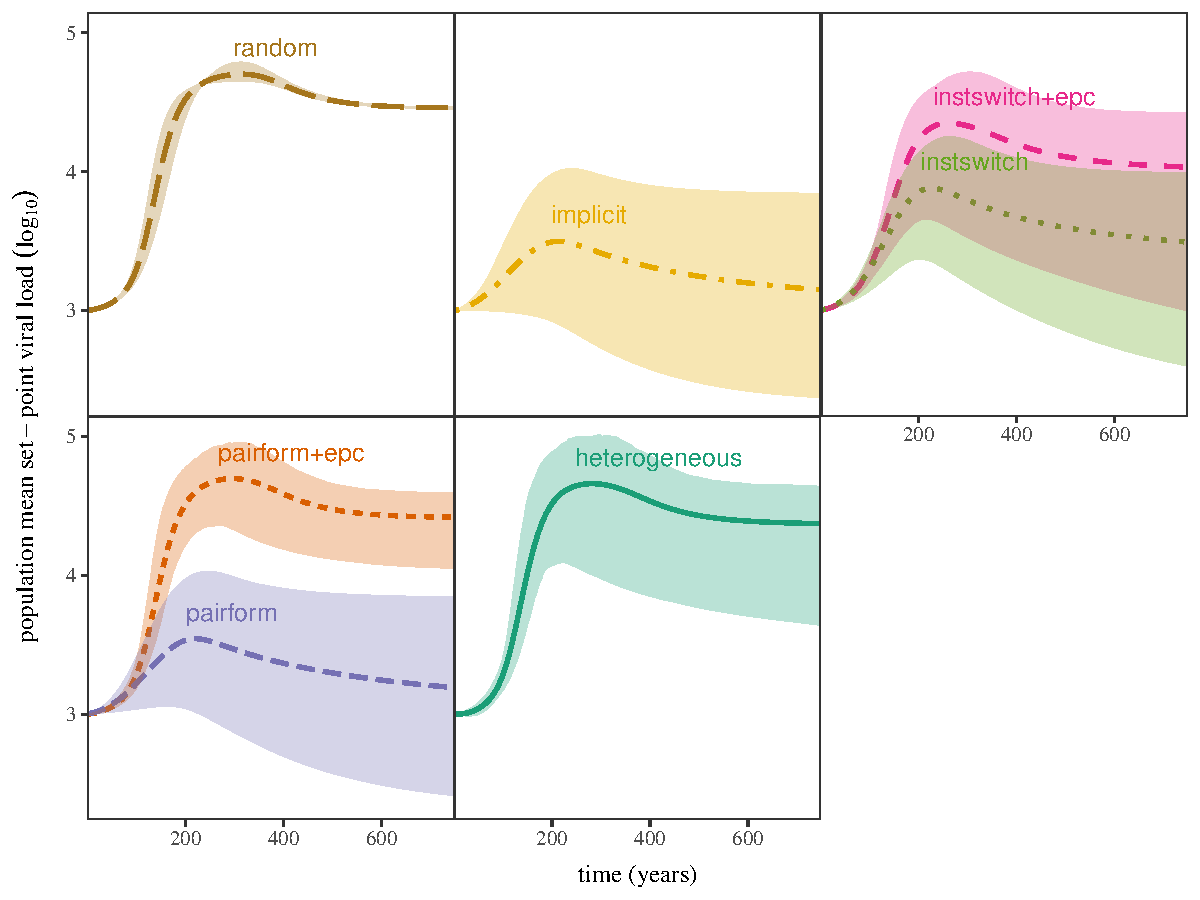
\includegraphics[width=\textwidth]{../figures/fig2.pdf}
\caption{{\bf Envelopes of virulence trajectories (population mean \Lspvl) under all models.}
All models were run until $t=4000~\textrm{years}$ using 1000 parameter sets obtained from Latin Hypercube Sampling to illustrate the range of dynamics each model can display. Envelope contains middle 95\% trajectories and lines within the envelope show mean trajectories. Truncated series are shown here.}
\label{fig:virtraj}
\end{figure}

Our chosen summary statistics (peak time, minimum expected progression time, equilibrium expected
progression time, and relative progression time) all vary considerably across models
(\figurename~\ref{fig:unidist}).
We first consider the models of intermediate realism: implicit,
instantaneous-switching with and without extra-pair contact, and
pair formation without extra-pair contact. Some parameter
sets for these models lead to low equilibrium virulence ($\approx 18$ years
to progression);
these same sets lead to correspondingly low
peak virulence (16 years to progression) and early peak times (before 200 years: \figurename~\ref{fig:pairplot}).
At the opposite extreme, parameter sets that produce high equilibrium virulence (8 years to progression)
also produce late peaks ($> 200~\text{years}$) and
high peak virulence (4 years to progression).
The pair-formation without extra-pair contact and implicit models
occasionally have parameter sets that select for such low virulence across
the board that they never exceed their initial virulence, leading to a tail
of peak times near zero.

\begin{figure}[!ht]
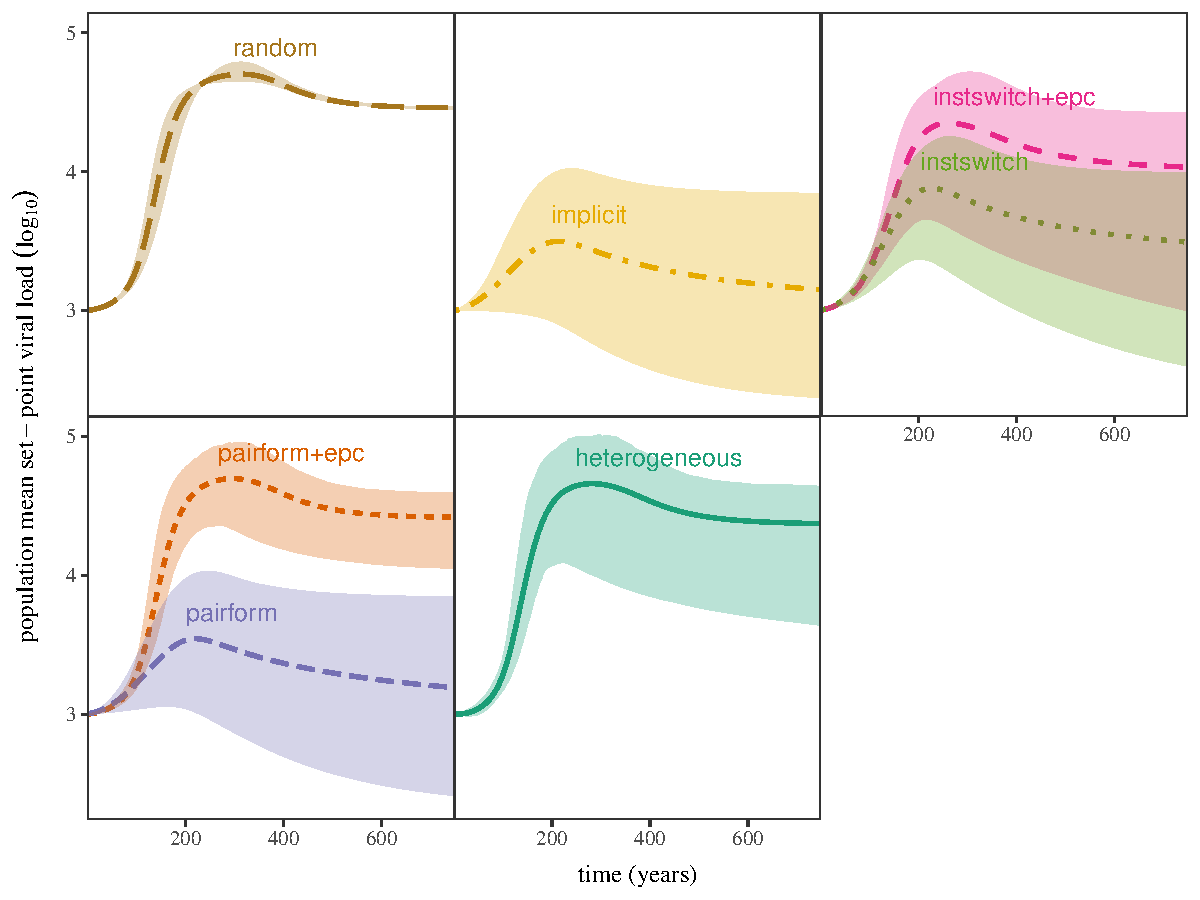
\includegraphics[width=\textwidth]{../figures/fig3.pdf}
\caption{{\bf Univariate distributions of summary statistics.}
For every simulation using LHS parameters, three summary statistics were obtained: peak time, maximum mean \Lspvl, and equilibrium mean \Lspvl.
Minimum mean progression time was obtained by by applying the hill function to maximum mean \Lspvl\ of each run.
The distribution of equilibrium mean \Lspvl\
(lower left panel) for the random mixing model is very narrow, and has been replaced by a point in order to preserve the vertical axis scaling.}
\label{fig:unidist}
\end{figure}

\begin{figure}[!ht]
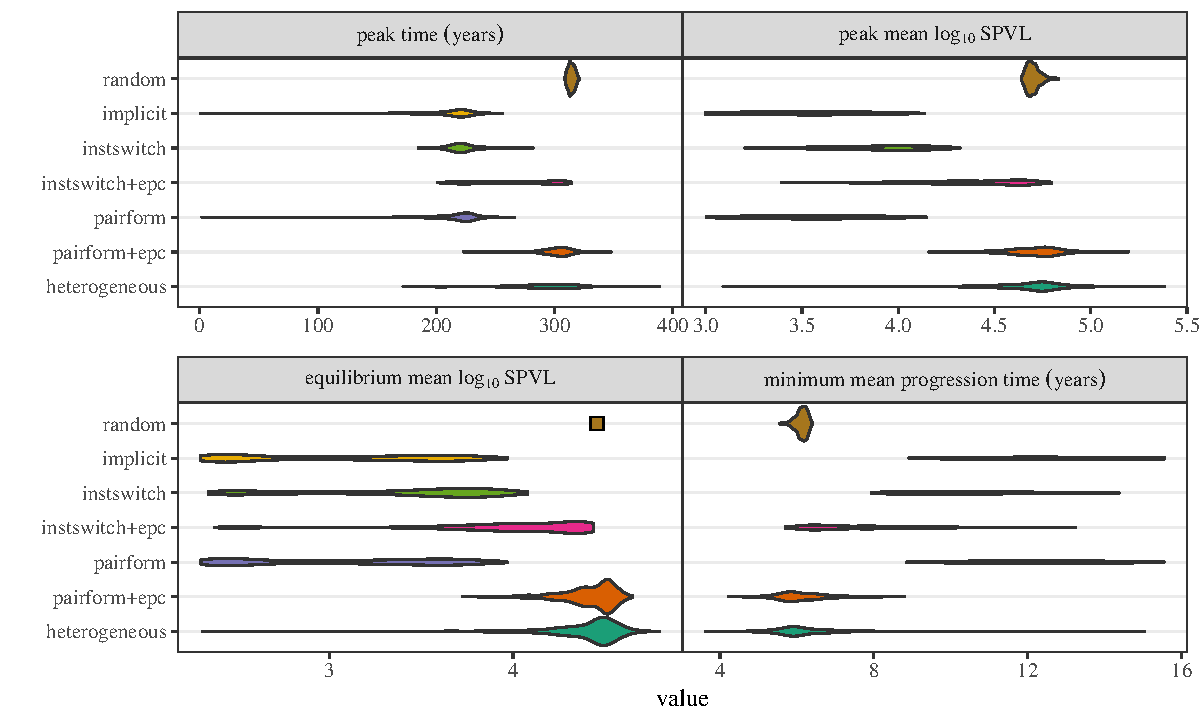
\includegraphics[width=\textwidth]{../figures/fig4.pdf}
\caption{{\bf Pairs plot: bivariate relationships among summary statistics for each model structure.}
Three summary statistics obtained from each simulation have been plotted against each other to visualize the relationship among the summary statistics.
All models follow a similar trend but each have distinguishing features.
Surprisingly, the implicit model, an approximation for instantaneous partnership formation model (instswitch), shows an almost identical trend with a model that has pair formation dynamics (pairform).
Dashed line in equilibrium vs. peak virulence plot shows 1:1 line, where equilibrium and peak virulence are equal.
100 values were sampled from each model to allow for clearer distinction between the models}
\label{fig:pairplot}
\end{figure}

The most striking aspect of the univariate comparisons in
\figurename~\ref{fig:unidist}, (and the bivariate comparisons in
\figurename~\ref{fig:pairplot}) is the similarity between the results of the
least (random mixing) and the most complex (pair formation with
extra-pair contact, pairform+epc with heterogeneity) models. The random-mixing model has the lowest variability, because it is unaffected by uncertainty in pair formation and extra-pair contact parameters, but otherwise the virulence
dynamics of these three extreme models are remarkably similar.
This phenomenon is driven by the strong effects of extra-pair contact in the
model with explicit pair formation and extra-pair contact 
(``pairform+epc'' in \figurename{}s~\ref{fig:virtraj}-\ref{fig:plot_sens}). When individuals spend time uncoupled between
partnerships, and when these single individuals can transmit disease
to coupled individuals, the resulting unstructured mixing overwhelms
the effect of structured mixing within couples, leading to mixing
that is effectively close to random.
Once unstructured mixing is strong, adding realistic heterogeneity
of mixing to the model has little effect other than increasing
the variability in the outcomes.

These differences are practically as well as 
scientifically important. The random-mixing, pairform+epc,
and heterogeneous models all predict rapid
progression to AIDS at the virulence peak
(median/95\% CI = 6.1 (5.7-6.3), 
6.02 (5.04-7.7), 6.03  (4.8-9.2)). 
In contrast, 
the implicit model predicts minimum progression times about twice as long:
12.5 (9.6-15.6) years. The corresponding differences in 
within-couple transmission
probability are even more extreme, about a fourfold difference:
0.249 (0.24-0.26), 0.252 (0.19-0.28), and 0.252 (0.15-0.28) per year for the 
random and pairform+epc models vs. 0.059 (0.02-0.13) per year
for the implicit model (see Appendix S2 for 
plots showing univariate summaries
of \Lspvl\ and transmission probability).

\begin{figure}[!ht]
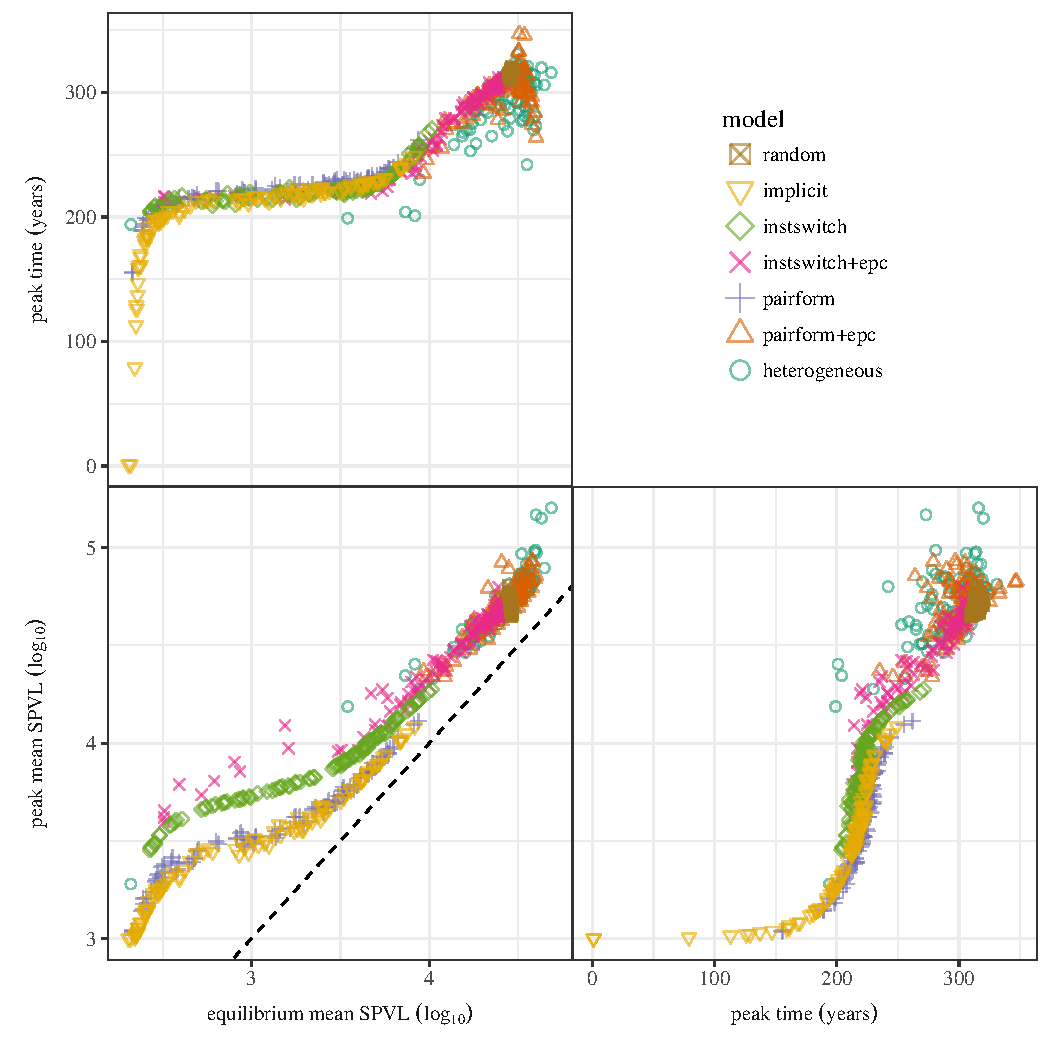
\includegraphics[width=\textwidth]{../figures/fig5.pdf}
\caption{{\bf Sensitivity plot.}
For most parameters in the Latin hypercube sample and each summary statistic, the figure shows the distribution (points) and trend (smooth line) of the summary statistic as a function of the parameter value, some of which have adjusted to achieve the standard initial epidemic growth rate (see Methods).}
Opposing trends in summary statistics with respect to partnership dissolution rate, $c$, (third column) between the model with and without extra-pair contact illustrates that similar model with different assumptions may yield opposing predictions.
\label{fig:plot_sens}
\end{figure}

The bivariate relationships (\figurename~\ref{fig:pairplot}) help distinguish the results of 
different models with similar univariate dynamical summaries. While the
relationship between equilibrium progression time and peak time is
similar for all model structures (top left panel), the other
relationships show more variation. In particular, the implicit
and pair-formation (without extra-pair contact) are very similar
to each other, but distinct from the other models. We still do
not have a convincing explanation for this distinction; we
would have expected the implicit model to be most similar to the
the instantaneous-switching model without extra-pair contact,
which most closely matches its derivation. However, we note
that the implicit model derivation is based on defining
the force of infection to match a scaled version of $\rzero$,
and as such would be expected to match the equilibrium behaviour
but not necessarily the epidemic-phase behaviour of a model
with explicit partnership dynamics.

Finally, the sensitivity plot (\figurename~\ref{fig:plot_sens}) shows the effects 
of each parameter on the summary statistics. 
The most notable difference can be observed by comparing the scaled parameters (e.g. $\beta_P$, $\beta_D$, $c$, $\rho$) with the unscaled parameters (e.g. $D_P$, $D_D$, $c_e/c_w$, $c_u/c_w$, $\kappa$, $\mu$);
note that the effects of $\beta_D$ and $D_D$ are not shown in \figurename~\ref{fig:plot_sens} as their patterns are so similar to $\beta_P$ and $D_P$, respectively.

One of the distinguishing features of the scaled parameters (in comparison to the unscaled parameters) is that the range of the parameters is compressed (relative to other models) for models without extra-pair contact as those models require parameters to be scaled by a large value in order to achieve a given $r$ of 0.04.
Models with extra-pair contact show wide range parameters as they can display a wide range of dynamics depending on $c_e/c_w$ (as well as $c_u/c_w$ for models with uncoupled mixing) and thus require wide range of scaling factors to achieve the target $r$.
Parameter range for random-mixing model is severely compressed because latin hypercube sampling does not affect the prevalence trajectory very much, and scaling factor does not vary much across parameters.

For parameters involved in partnership turnover ($c$ and $\rho$), main distinction is between models with and without extra-pair contact. With extra-pair contact, we get gradual decrease in peak time, maximum \Lspvl, and equilibrium \Lspvl\ with increasing turnover rates; Otherwise we get increase in summary statistics.
Although we have not verified this idea analytically, we speculate that increase in turnover rates diminishes the effect of epc (equivalently increasing relative importance of within-partnership contact), therefore selecting for lower \Lspvl.
For models without epc, increased rates of partnership change decrease the level of structured mixing (mimicing epc models), resulting in selection for higher \Lspvl.

We also note that the implicit model and the instantaneous partnership formation model show similar patterns in scaled parameters. In fact, we can see that the effect of partnership dissolution rate, $c$, on equilibrium \Lspvl\ of the two models are almost identical (in \figurename~\ref{fig:pairplot}, they have distinguishing features).
Lastly, we note that increase in transmission rates ($\beta_P$ and $\beta_D$) has a decreasing effect on summary statistics for all models except for random mixing model.

Surprisingly, once calibration
is taken into account, the unscaled parameters have little to no effect overall.
Increase in duration ($D_P$, $D_D$) in the primary and disease stages generally decrease the equilibrium virulence, peak virulence, and peak time,
although the models with uncoupled mixing and random mixing model have high, relatively
constant values with respect to these parameters.
The ratio of extra-pair to within-pair contact ($c_e/c_w$) affects
summary statistics in the instantaneous-switching +epc model, but not the pair-formation+epc
model (probably because the uncoupled individuals present in the pair-formation+epc
model make extra-pair contact by coupled individuals less important).
Similarly, increasing the ratio of uncoupled to within-pair contact, $c_u/c_w$, increases peak and equilibrium \Lspvl\ and delays peak time of the pair-formation+epc model but has almost no effect on the heterogeneous model.
Neither the uncoupled contact rate nor
the mean ($\mu$) or CV$^2$ of the number of non-cohabiting sexual
partners has much systematic effect in the heterogeneous model.

\section*{Discussion}

All models must simplify the world.  Many constraints --- among them data
availability, computation time, and code complexity --- drive the need
for parsimony, with different constraints applying in different
contexts. The critical question that modelers must ask is whether the
simplified model gives adequate answers, or whether the
simplifications lead to qualitative or quantitative errors.
This question is especially important for modelers who
are hoping that their conclusions will guide management decisions.

In the particular example of HIV virulence eco-evolutionary dynamics
and the complexity of contact structures
we reach the slightly ironic conclusion that the
effort put into building a more realistic model essentially cancels
out, putting us back where we started when used a naive random-mixing
contact model.
However, we are not quite back where we started, as the
complex models lead to wider, presumably more realistic
confidence intervals on the predictions.
In general, unstructured mixing --- whether occurring through 
purely random mixing, or through extra-pair contact and contact
among people outside of stable partnerships --- tends to drive
faster virulence evolution, leading to higher peak virulence and 
lower times to progression at the peak time.

%In Herbeck \etal's \cite{herbeck_hiv_2014} network model of partnerships, the partnership duration is set to 1 day --- very unrealistic in epidemic terms, but perhaps
%actually more true to real-world HIV epidemiological dynamics than a
%model with realistic partnership durations that neglects extra-pair
%contact \cite{herbeck2016evolution}. 
Taking further steps to make the model even more realistic
might add further structure,
making the random-mixing model predictions less accurate. For
example, our model forms partnerships randomly, and assumes that
extra-pair contact is randomly mixing across the population;
one could instead model extra-pair contact as arising from
multiple concurrent partnerships (some, such as contact with sex
workers, of very short duration) and/or more structured partnership
formation (by age, ethnicity, or behaviour group). The effects of
other realistic complications such as explicit modeling of two
sexes (both in contact structure and differential transmission
probabilities), temporal and spatial variation in epidemic processes,
or presence of genetic variation in hosts are harder to predict.

Parameterization is one of the biggest challenges of epidemiological
modeling. In addition to following Champredon \etal\ \cite{champredon_hiv_2013} 
by doing Latin hypercube
sampling across a wide range of epidemiological parameters, we 
calibrated each set of parameters to the same initial epidemic
growth rate, chosen to match the results of previous models
\cite{shirreff_transmission_2011}.  Previous models 
in this area have drawn their
parameters from cohort studies from the 1990s
\cite{wawer2005rates,hollingsworth_hiv1_2008}
rather than doing any explicit calibration to epidemic curves,
but they give reasonable order-of-magnitude
growth rates ($\approx 0.04~\textrm{year}^{-1}$)
for the early stages of the HIV epidemic (although considerably
lower than estimates of $\approx 0.07-0.1~\textrm{year}^{-1}$
based on population genetic reconstructions \cite{faria_early_2014}).
However, our reason for calibrating was not to match any
specific observed epidemic, but rather to make sure that
we were making meaningful comparisons across a range of
models with radically different contact structures, and
hence involving different interpretations of the same quantitative
parameters.  For example, in models with instantaneous switching the
partnership dissolution rate $c$ is identical to the partnership
formation rate; in models with explicit partnership formation,
the partnership formation rate is also $c$ at equilibrium,
but might vary over the course of an epidemic.
It is not obvious whether models with equal parameters but
different structures should be directly compared; calibration
solves this problem.

More generally, any model that wants to be
taken seriously for management and forecasting purposes should
be calibrated to \emph{all} available data, using informative
priors to incorporate both realistic distributions of uncertainty
for all parameters from independent measurements \cite{elderd_uncertainty_2006}
and calibration from population-level observations of epidemic
trajectories. Such a procedure would also be an improvement on the common --- although not universal --- %
practice, which we have followed here,
of assessing uncertainty over uniform ranges rather than
using distributions that allow more continuous variation in support over
the range of a parameter.

Researchers have documented that HIV virulence and set-point viral
load are changing, on time scales comparable to those portrayed here
(e.g., compare \figurename~\ref{fig:virtraj} to Herbeck \etal's
estimated rate of change of 1.3 \Lspvl\ per century [95\% CI -0.1 to
  3] \cite{herbeck_is_2012}), and have begun to build relatively realistic models that
attempt to describe how interventions such as mass antiretroviral
therapy (ART) can be expected to change the trajectory of virulence
evolution \cite{payne_impact_2014,roberts2015impact,herbeck_evolution_2016}.  While these
efforts are well-intentioned, we caution that 
structural details that are currently omitted from these models
could significantly change their conclusions.

\section*{Acknowledgements}
We would like to thank Christophe Fraser and
David Champredon for access to simulation code
and Wim Delva and an anonymous reviewer for useful comments;
this work was funded by NSERC Discovery Grant 386590-2010.
Computational resources were provided by SHARCnet.

\section*{Supporting Information}

% Include only the SI item label in the paragraph heading. Use the \nameref{label} command to cite SI items in the text.
\paragraph*{Appendix S1: Model Details}
\label{S1_Appendix}

\paragraph*{Appendix S2: Dynamics of Transmission and Virulence}

\label{S2_Appendix}

\clearpage

\nolinenumbers

% Either type in your references using
% \begin{thebibliography}{}
% \bibitem{}
% Text
% \end{thebibliography}
%
% or
%
% Compile your BiBTeX database using our plos2015.bst
% style file and paste the contents of your .bbl file
% here.
% 

\begin{thebibliography}{10}

\bibitem{alizon_virulence_2009}
Alizon S, Hurford A, Mideo N, van Baalen M.
\newblock Virulence evolution and the trade-off hypothesis: history, current
  state of affairs and the future.
\newblock J Evol Biol. 2009;22:245--259.
\newblock doi:{10.1111/j.1420-9101.2008.01658.x}.

\bibitem{EbertBull2003}
Ebert D, Bull JJ.
\newblock Challenging the trade-off model for the evolution of virulence: is
  virulence management feasible?
\newblock Trends Microbiol. 2003;11(1):15--20.

\bibitem{alizon_adaptive_2015}
Alizon S, Michalakis Y.
\newblock Adaptive virulence evolution: the good old fitness-based approach.
\newblock Trends in Ecology \& Evolution. 2015;30(5):248--254.
\newblock doi:{10.1016/j.tree.2015.02.009}.

\bibitem{Dwyer+1990}
Dwyer G, Levin SA, Buttel L.
\newblock A simulation model of the population dynamics and evolution of
  myxomatosis.
\newblock Ecol Monog. 1990;60:423--447.

\bibitem{mackinnon1999genetic}
Mackinnon MJ, Read AF.
\newblock Genetic relationships between parasite virulence and transmission in
  the rodent malaria {{\em Plasmodium chabaudi}}.
\newblock Evolution. 1999; p. 689--703.

\bibitem{jensen2006empirical}
Jensen KH, Little T, Skorping A, Ebert D.
\newblock Empirical support for optimal virulence in a castrating parasite.
\newblock PLoS Biol. 2006;4(7):e197.

\bibitem{deroode2008virulence}
De~Roode JC, Yates AJ, Altizer S.
\newblock Virulence-transmission trade-offs and population divergence in
  virulence in a naturally occurring butterfly parasite.
\newblock Proceedings of the National Academy of Sciences.
  2008;105(21):7489--7494.

\bibitem{Fraser+2007}
Fraser C, Hollingsworth TD, Chapman R, de~Wolf F, Hanage WP.
\newblock Variation in {HIV}-1 set-point viral load: Epidemiological analysis
  and an evolutionary hypothesis.
\newblock PNAS. 2007;104:17441--17446.

\bibitem{fraser_virulence_2014}
Fraser C, Lythgoe K, Leventhal GE, Shirreff G, Hollingsworth TD, Alizon S,
  et~al.
\newblock Virulence and Pathogenesis of {HIV}-1 Infection: An Evolutionary
  Perspective.
\newblock Science. 2014;343(6177):1243727.
\newblock doi:{10.1126/science.1243727}.

\bibitem{shirreff_transmission_2011}
Shirreff G, Pellis L, Laeyendecker O, Fraser C.
\newblock Transmission Selects for {HIV-1} Strains of Intermediate Virulence: A
  Modelling Approach.
\newblock PLoS Computational Biology. 2011;7(10):e1002185.
\newblock doi:{10.1371/journal.pcbi.1002185}.

\bibitem{herbeck_hiv_2014}
Herbeck JT, Mittler JE, Gottlieb GS, Mullins JI.
\newblock An {HIV} Epidemic Model Based on Viral Load Dynamics: Value in
  Assessing Empirical Trends in {HIV} Virulence and Community Viral Load.
\newblock {PLoS} Comput Biol. 2014;10(6):e1003673.

\bibitem{herbeck_evolution_2016}
Herbeck JT, Mittler JE, Gottlieb GS, Goodreau SM, Murphy JT, Cori A, et~al.
\newblock Evolution of {HIV} virulence in response to widespread scale up of
  antiretroviral therapy: a modeling study.
\newblock Virus Evolution. 2016;2(2):vew028.
\newblock doi:{10.1093/ve/vew028}.

\bibitem{day_virulence_2004}
Day T, Proulx SR.
\newblock A General Theory for the Evolutionary Dynamics of Virulence.
\newblock The American Naturalist. 2004;163(4):E40--E63.
\newblock doi:{10.1086/382548}.

\bibitem{alizon_price_2009}
Alizon S.
\newblock The {Price} equation framework to study disease within-host
  evolution.
\newblock Journal of Evolutionary Biology. 2009;22(5):1123--1132.
\newblock doi:{10.1111/j.1420-9101.2009.01726.x}.

\bibitem{champredon_hiv_2013}
Champredon D, Bellan S, Dushoff J.
\newblock {HIV} Sexual Transmission Is Predominantly Driven by Single
  Individuals Rather than Discordant Couples: A Model-Based Approach.
\newblock PLoS ONE. 2013;8(12):e82906.
\newblock doi:{10.1371/journal.pone.0082906}.

\bibitem{dietz_epidemiological_1988}
Dietz K, Hadeler KP.
\newblock Epidemiological models for sexually transmitted diseases.
\newblock Journal of Mathematical Biology. 1988;26(1):1--25.

\bibitem{kretzschmar_effect_1998}
Kretzschmar M, Dietz K.
\newblock The effect of pair formation and variable infectivity on the spread
  of an infection without recovery.
\newblock Mathematical Biosciences. 1998;148(1):83--113.

\bibitem{hollingsworth_hiv1_2008}
Hollingsworth TD, Anderson RM, Fraser C.
\newblock {HIV}-1 Transmission, by Stage of Infection.
\newblock Journal of Infectious Diseases. 2008;198(5):687--693.
\newblock doi:{10.1086/590501}.

\bibitem{omori2015dynamics}
Omori R, Chemaitelly H, Abu-Raddad LJ.
\newblock Dynamics of non-cohabiting sex partnering in sub-{Saharan} {Africa}:
  a modelling study with implications for {HIV} transmission.
\newblock Sexually Transmitted Infections.
  2015;doi:{10.1136/sextrans-2014-051925}.

\bibitem{may_transmission_1988}
May RM, Anderson RM.
\newblock The Transmission Dynamics of Human Immunodeficiency Virus (HIV).
\newblock Philosophical Transactions of the Royal Society of London Series B,
  Biological Sciences. 1988;321(1207):565--607.

\bibitem{delva_connecting_2016}
Delva W, Leventhal GE, Helleringer S.
\newblock Connecting the dots: network data and models in {HIV} epidemiology.
\newblock AIDS. 2016;30(13):2009--2020.
\newblock doi:{10.1097/QAD.0000000000001184}.

\bibitem{blower_drugs_1991}
Blower SM, Hartel D, Dowlatabadi H, Anderson RM, May RM.
\newblock Drugs, Sex and {HIV}: A Mathematical Model for {New York City}.
\newblock Philosophical Transactions of the Royal Society of London B:
  Biological Sciences. 1991;331(1260):171--187.
\newblock doi:{10.1098/rstb.1991.0006}.

\bibitem{ma_estimating_2014}
Ma J, Dushoff J, Bolker BM, Earn DJD.
\newblock Estimating Initial Epidemic Growth Rates.
\newblock Bulletin of Mathematical Biology. 2014;76(1):245--260.
\newblock doi:{10.1007/s11538-013-9918-2}.

\bibitem{wallinga_how_2007}
Wallinga J, Lipsitch M.
\newblock How generation intervals shape the relationship between growth rates
  and reproductive numbers.
\newblock Proceedings of the Royal Society of London B: Biological Sciences.
  2007;274(1609):599--604.
\newblock doi:{10.1098/rspb.2006.3754}.

\bibitem{soetaert_solving_2010}
Soetaert K, Petzoldt T, Setzer RW.
\newblock Solving Differential Equations in {R}: Package {deSolve}.
\newblock Journal of Statistical Software. 2010;33(9):1--25.
\newblock doi:{10.18637/jss.v033.i09}.

\bibitem{wawer2005rates}
Wawer MJ, Gray RH, Sewankambo NK, Serwadda D, Li X, Laeyendecker O, et~al.
\newblock Rates of {HIV}-1 transmission per coital act, by stage of {HIV}-1
  infection, in {Rakai}, {Uganda}.
\newblock Journal of Infectious Diseases. 2005;191(9):1403--1409.

\bibitem{faria_early_2014}
Faria NR, Rambaut A, Suchard MA, Baele G, Bedford T, Ward MJ, et~al.
\newblock The early spread and epidemic ignition of {HIV}-1 in human
  populations.
\newblock Science (New York, NY). 2014;346(6205):56--61.
\newblock doi:{10.1126/science.1256739}.

\bibitem{elderd_uncertainty_2006}
Elderd BD, Dukic VM, Dwyer G.
\newblock Uncertainty in predictions of disease spread and public health
  responses to bioterrorism and emerging diseases.
\newblock Proceedings of the National Academy of Sciences. 2006;103(42):15693
  --15697.
\newblock doi:{10.1073/pnas.0600816103}.

\bibitem{herbeck_is_2012}
Herbeck JT, Müller V, Maust BS, Ledergerber B, Torti C, Di~Giambenedetto S,
  et~al.
\newblock Is the virulence of {HIV} changing? {A} meta-analysis of trends in
  prognostic markers of {HIV} disease progression and transmission.
\newblock AIDS (London, England). 2012;26(2):193--205.
\newblock doi:{10.1097/QAD.0b013e32834db418}.

\bibitem{payne_impact_2014}
Payne R, Muenchhoff M, Mann J, Roberts HE, Matthews P, Adland E, et~al.
\newblock Impact of {HLA}-driven {HIV} adaptation on virulence in populations
  of high {HIV} seroprevalence.
\newblock Proceedings of the National Academy of Sciences.
  2014;111(50):E5393--E5400.
\newblock doi:{10.1073/pnas.1413339111}.

\bibitem{roberts2015impact}
Roberts HE, Goulder PJ, McLean AR.
\newblock The impact of antiretroviral therapy on population-level virulence
  evolution of {HIV}-1.
\newblock Journal of The Royal Society Interface. 2015;12(113):20150888.

\end{thebibliography}
\end{document}

